% ============================================================================
%  CHAPTER 6 — SYSTEM ARCHITECTURE
% ============================================================================
\chapter{System Architecture}
\label{ch:architecture}

\epigraph{Architecture is the allocation of responsibilities to components and the definition of the interfaces between them.}{}

This chapter presents the complete system architecture: what runs where, how the components communicate, and why the design is structured as it is.

% ────────────────────────────────────────────────────────────────────────────
\section{The ``Bump in the Wire'' Concept}
\label{sec:arch-bump}

The secure tunnel operates as a \textbf{transparent proxy}---a ``bump in the wire'' between the application (Mission Planner or MAVProxy) and the physical network. Neither the application nor the flight controller knows the tunnel exists:

\begin{itemize}
  \item The application sends plaintext UDP datagrams to a \emph{local} port.
  \item The proxy encrypts them and sends them over the network.
  \item On the far end, the peer proxy decrypts them and delivers plaintext to the application.
\end{itemize}

No code changes are required in MAVLink applications, flight controllers, or ground station software. The only configuration change is redirecting the application's connection to the proxy's local port instead of the remote peer's network port.

% ────────────────────────────────────────────────────────────────────────────
\section{Hardware Topology}
\label{sec:arch-hardware}

The system consists of two physical nodes connected by a WiFi network:

\begin{figure}[htbp]
  \centering
  \begin{tikzpicture}[
    node distance=3cm,
    box/.style={draw, rounded corners, minimum width=3.5cm, minimum height=1.5cm, align=center, font=\small},
    hw/.style={draw, rounded corners, minimum width=2.5cm, minimum height=1cm, align=center, fill=blue!10, font=\small},
    link/.style={->, thick}
  ]
    % Drone side
    \node[hw] (pixhawk) {Pixhawk 6C\\Flight Controller};
    \node[hw, below=1.5cm of pixhawk] (pi) {Raspberry Pi 5\\(8\,GB RAM)};
    \node[box, below=1.5cm of pi] (droneproxy) {Drone Proxy\\{\footnotesize\texttt{core/async\_proxy.py}}};
    
    % GCS side
    \node[hw, right=6cm of pixhawk] (laptop) {Windows Laptop\\(i7, 32\,GB RAM)};
    \node[box, below=1.5cm of laptop] (mp) {Mission Planner\\or MAVProxy};
    \node[box, below=1.5cm of mp] (gcsproxy) {GCS Proxy\\{\footnotesize\texttt{core/async\_proxy.py}}};
    
    % Connections
    \draw[link] (pixhawk) -- node[right, font=\footnotesize] {USB Serial} (pi);
    \draw[link] (pi) -- node[right, font=\footnotesize, align=center] {MAVProxy\\UDP} (droneproxy);
    \draw[link] (laptop) -- node[right, font=\footnotesize] {UDP} (mp);
    \draw[link] (mp) -- node[right, font=\footnotesize] {UDP} (gcsproxy);
    
    % WiFi link
    \draw[<->, very thick, red!70!black] (droneproxy) -- node[below, font=\footnotesize] {WiFi: TCP + UDP (encrypted)} (gcsproxy);
    
    % Optional INA219
    \node[hw, left=1.5cm of pi, yshift=-0.5cm] (ina) {INA219\\Power Sensor};
    \draw[link, dashed] (ina) -- node[above, font=\tiny] {I2C} (pi);
  \end{tikzpicture}
  \caption{Physical hardware topology of the secure tunnel system.}
  \label{fig:hardware-topology}
\end{figure}

\subsection{Drone Side (Raspberry Pi 5)}

\begin{itemize}
  \item \textbf{Raspberry Pi 5} (8\,GB): Runs the drone proxy, MAVProxy, and benchmark orchestrator.
  \item \textbf{Pixhawk 6C}: The flight controller, connected via USB serial. Outputs MAVLink telemetry and accepts commands.
  \item \textbf{INA219 Power Sensor} (optional): Connected via I2C, measures current and voltage for power benchmarking.
  \item \textbf{WiFi}: The Pi's built-in WiFi (\texttt{wlan0}) or a USB WiFi adapter.
\end{itemize}

\subsection{GCS Side (Windows Laptop)}

\begin{itemize}
  \item \textbf{Windows PC}: Runs the GCS proxy, Mission Planner (or MAVProxy), and optionally the analysis dashboard.
  \item \textbf{Python + conda}: The \texttt{oqs-dev} conda environment provides \texttt{oqs-python} with PQC support.
\end{itemize}

% ────────────────────────────────────────────────────────────────────────────
\section{Network Port Map}
\label{sec:arch-ports}

Every network socket in the system has a precisely defined role:

\begin{table}[htbp]
  \centering
  \caption{Complete network port map.}
  \label{tab:port-map}
  \small
  \begin{tabular}{lllcl}
    \toprule
    \textbf{Side} & \textbf{Bind Address} & \textbf{Protocol} & \textbf{Port} & \textbf{Purpose} \\
    \midrule
    GCS   & \texttt{0.0.0.0}   & TCP & 46000 & Handshake server (listens) \\
    GCS   & \texttt{0.0.0.0}   & UDP & 46011 & Encrypted RX (from drone) \\
    GCS   & \texttt{127.0.0.1} & UDP & 47001 & Plaintext TX (app $\to$ proxy) \\
    GCS   & \texttt{127.0.0.1} & UDP & 47002 & Plaintext RX (proxy $\to$ app) \\
    \midrule
    Drone & connects to GCS    & TCP & $\to$46000 & Handshake client \\
    Drone & \texttt{0.0.0.0}   & UDP & 46012 & Encrypted RX (from GCS) \\
    Drone & \texttt{127.0.0.1} & UDP & 47003 & Plaintext TX (MAVProxy $\to$ proxy) \\
    Drone & \texttt{127.0.0.1} & UDP & 47004 & Plaintext RX (proxy $\to$ MAVProxy) \\
    \midrule
    Drone & \texttt{0.0.0.0}   & TCP & 48080 & Control channel (scheduler) \\
    \bottomrule
  \end{tabular}
\end{table}

\begin{designdecision}
Plaintext ports bind to \texttt{127.0.0.1} (localhost only), ensuring that unencrypted MAVLink traffic never leaves the local machine. Encrypted ports bind to \texttt{0.0.0.0} (all interfaces), allowing the peer to reach them over WiFi. This is a deliberate security measure.
\end{designdecision}

% ────────────────────────────────────────────────────────────────────────────
\section{The Three Communication Planes}
\label{sec:arch-planes}

The system uses three distinct communication planes:

\subsection{Control Plane (TCP)}

\begin{description}
  \item[Handshake channel (TCP 46000):] Used exclusively for the PQC key exchange. The drone connects as TCP client; the GCS listens as TCP server. Traffic is minimal (a few kilobytes per handshake) but latency-sensitive: the data plane cannot operate until the handshake completes.
  
  \item[Scheduler control channel (TCP 48080):] Used by the benchmark orchestrator. The drone controller sends JSON commands (``start proxy,'' ``switch suite,'' ``stop'') to the GCS follower. This channel carries no MAVLink traffic.
\end{description}

\subsection{Data Plane (UDP, encrypted)}

The high-throughput path. Encrypted MAVLink datagrams flow bidirectionally between the drone (port~46012) and GCS (port~46011). Every packet carries the 22-byte AEAD header and 16-byte authentication tag.

\subsection{Plaintext Plane (UDP, localhost)}

The loopback path between the proxy and local applications. On the drone: MAVProxy $\leftrightarrow$ proxy on ports 47003/47004. On the GCS: Mission Planner $\leftrightarrow$ proxy on ports 47001/47002. This traffic \textbf{never} leaves the local machine.

\begin{figure}[htbp]
  \centering
  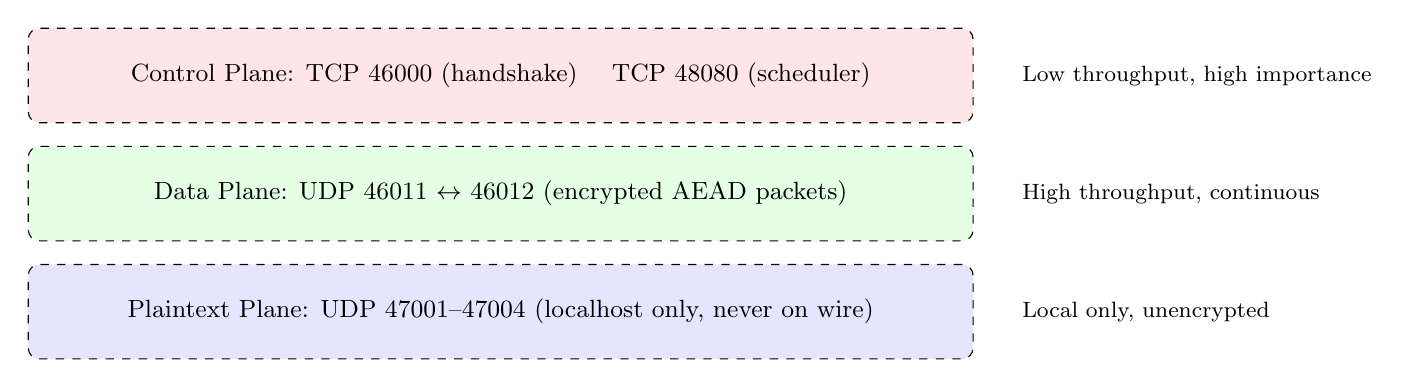
\begin{tikzpicture}[
    plane/.style={draw, dashed, rounded corners, minimum width=12cm, minimum height=1.2cm, font=\small},
    arr/.style={<->, thick}
  ]
    \node[plane, fill=red!10]   (ctrl)  at (0,3) {Control Plane: TCP 46000 (handshake) \quad TCP 48080 (scheduler)};
    \node[plane, fill=green!10] (data)  at (0,1.5) {Data Plane: UDP 46011 $\leftrightarrow$ 46012 (encrypted AEAD packets)};
    \node[plane, fill=blue!10]  (plain) at (0,0) {Plaintext Plane: UDP 47001--47004 (localhost only, never on wire)};
    
    \node[font=\footnotesize, right] at (6.5,3)   {Low throughput, high importance};
    \node[font=\footnotesize, right] at (6.5,1.5) {High throughput, continuous};
    \node[font=\footnotesize, right] at (6.5,0)   {Local only, unencrypted};
  \end{tikzpicture}
  \caption{The three communication planes of the secure tunnel.}
  \label{fig:three-planes}
\end{figure}

% ────────────────────────────────────────────────────────────────────────────
\section{Software Components}
\label{sec:arch-components}

The codebase is organized into three major directories, each with a clear responsibility:

\subsection{\texttt{core/} --- The Tunnel Engine}

This is the security-critical core: the proxy, handshake, AEAD framing, and suite registry. It runs on \textbf{both} drone and GCS, using the same code with different configuration.

\begin{table}[htbp]
  \centering
  \caption{Key modules in \texttt{core/}.}
  \label{tab:core-modules}
  \small
  \begin{tabular}{lp{9cm}}
    \toprule
    \textbf{Module} & \textbf{Responsibility} \\
    \midrule
    \texttt{config.py}          & Single source of truth: all ports, IPs, feature flags, timeouts \\
    \texttt{async\_proxy.py}    & Main event loop (selectors-based). Manages 4 UDP sockets, handshake, encrypt/decrypt, rate limiting, rekey \\
    \texttt{handshake.py}       & PQC handshake: KEM keygen/encap/decap, SIG sign/verify, HKDF key derivation, HMAC drone auth \\
    \texttt{aead.py}            & AEAD framing: Sender (encrypt + header), Receiver (validate + decrypt + anti-replay) \\
    \texttt{suites.py}          & Suite registry: KEM$\times$AEAD$\times$SIG Cartesian product, alias resolution, runtime probing \\
    \texttt{run\_proxy.py}      & CLI entry point: \texttt{init-identity}, \texttt{gcs}, \texttt{drone} subcommands \\
    \texttt{policy\_engine.py}  & Two-phase commit rekey state machine (IDLE$\to$PREPARE\_SENT$\to$COMMITTED/ABORTED) \\
    \texttt{metrics\_aggregator.py} & Central metrics orchestrator: wires all collectors, thread-safe sampling \\
    \texttt{metrics\_schema.py} & 18-category metrics schema definition (categories A through R) \\
    \texttt{power\_monitor.py}  & INA219 I2C power measurement with sign auto-detection and CSV logging \\
    \texttt{mavlink\_collector.py} & Passive MAVLink sniffer: message rates, heartbeat tracking, sequence gaps \\
    \texttt{process.py}         & Managed subprocess with Windows Job Objects / Linux PDEATHSIG cleanup \\
    \bottomrule
  \end{tabular}
\end{table}

\subsection{\texttt{sscheduler/} --- The Benchmark Orchestrator}

The ``simplified scheduler'' manages automated benchmark runs. The \textbf{drone} is the controller; the \textbf{GCS} is the follower.

\begin{table}[htbp]
  \centering
  \caption{Key modules in \texttt{sscheduler/}.}
  \label{tab:sscheduler-modules}
  \small
  \begin{tabular}{lp{9cm}}
    \toprule
    \textbf{Module} & \textbf{Responsibility} \\
    \midrule
    \texttt{sdrone\_bench.py} & Drone benchmark controller: manages GCS via TCP, cycles suites, collects metrics, writes JSONL \\
    \texttt{sgcs\_bench.py}   & GCS benchmark follower: starts/stops proxy and MAVProxy per instructions from drone \\
    \texttt{sdrone\_mav.py}   & Drone MAVProxy management: serial port detection, process lifecycle \\
    \texttt{sgcs\_mav.py}     & GCS MAVProxy management \\
    \texttt{benchmark\_policy.py} & BenchmarkPolicy: \funcname{evaluate()} (proposal, no side effects) + \funcname{confirm\_advance()} (state mutation) \\
    \texttt{policy.py}        & Runtime policies: TelemetryAwarePolicy (safety-critical), SequentialPolicy, RandomPolicy \\
    \bottomrule
  \end{tabular}
\end{table}

\subsection{\texttt{dashboard/} --- The Analysis Dashboard}

A web-based visualization tool for benchmark results.

\begin{description}
  \item[Backend:] FastAPI (Python), Pydantic v2 models, JSONL/JSON ingestion from benchmark outputs.
  \item[Frontend:] React 18 + TypeScript + Vite, Zustand state management, Recharts for visualization, TailwindCSS for styling.
\end{description}

The dashboard is covered in detail in Chapter~\ref{ch:dashboard}.

% ────────────────────────────────────────────────────────────────────────────
\section{End-to-End Data Flow}
\label{sec:arch-dataflow}

This section traces a single MAVLink packet from the Pixhawk to Mission Planner:

\begin{enumerate}
  \item \textbf{Pixhawk $\to$ Pi (serial):} The flight controller sends a MAVLink telemetry packet over USB serial.
  
  \item \textbf{MAVProxy (Pi):} Reads the serial frame, produces a UDP datagram, sends it to \texttt{127.0.0.1:47003}.
  
  \item \textbf{Drone Proxy ingress:} The proxy's selectors loop detects a readable event on the plaintext socket. It reads the datagram (e.g., 50 bytes of MAVLink).
  
  \item \textbf{Encryption:} The proxy calls \funcname{Sender.encrypt()}, which:
  \begin{itemize}
    \item Constructs a 22-byte header (version, algorithm IDs, session ID, sequence number, epoch).
    \item Derives the nonce from epoch + sequence.
    \item Calls the AEAD algorithm (e.g., AES-256-GCM) to encrypt the 50 bytes and produce a 16-byte tag, using the header as AAD.
    \item Returns the 88-byte wire packet (22 header + 50 ciphertext + 16 tag).
  \end{itemize}
  
  \item \textbf{Transmission:} The proxy sends the 88-byte UDP datagram from the drone's network interface to the GCS at \texttt{<GCS\_IP>:46011}.
  
  \item \textbf{GCS Proxy ingress:} The GCS proxy's selectors loop detects a readable event on the encrypted socket. It reads the 88-byte datagram.
  
  \item \textbf{Decryption:} The proxy calls \funcname{Receiver.decrypt()}, which:
  \begin{itemize}
    \item Parses and validates the 22-byte header (version, algorithm IDs, session ID match).
    \item Checks the replay window (is this sequence number new?).
    \item Reconstructs the nonce from epoch + sequence.
    \item Calls the AEAD algorithm to decrypt and verify the tag.
    \item If authentication fails: drops the packet silently.
    \item If authentication succeeds: returns the 50-byte plaintext.
  \end{itemize}
  
  \item \textbf{GCS Proxy egress:} Sends the 50-byte plaintext datagram to \texttt{127.0.0.1:47002}.
  
  \item \textbf{Mission Planner:} Receives the datagram on port 47002, parses it as MAVLink, and displays the telemetry on the HUD.
\end{enumerate}

Return traffic (commands from Mission Planner to the Pixhawk) follows the same path in reverse, using the \texttt{key\_gcs\_to\_drone} symmetric key instead of \texttt{key\_drone\_to\_gcs}.

\begin{keyinsight}
The entire encryption/decryption path adds approximately 30--200 microseconds of latency per packet, depending on the AEAD algorithm. For a typical MAVLink stream of 50 messages/second, this overhead is negligible compared to WiFi latency ($\sim$1--5\,ms).
\end{keyinsight}

% ────────────────────────────────────────────────────────────────────────────
\section{Trust Model}
\label{sec:arch-trust}

The system's trust model defines what each party needs to know before communication begins:

\begin{description}
  \item[GCS has:] A long-term signature key pair (private + public). Generated once via \texttt{python -m core.run\_proxy init-identity}.
  
  \item[Drone has:] The GCS's \textbf{public} signature key (pre-installed), plus a \textbf{pre-shared key (PSK)} for drone authentication.
  
  \item[Pre-shared key (PSK):] A symmetric secret known to both sides, used during the handshake for the drone to prove its identity via HMAC. This is set via the \configkey{DRONE\_PSK} configuration key.
\end{description}

\begin{securitynote}
The trust model is asymmetric: the GCS authenticates via digital signature (the drone verifies the GCS's public key), and the drone authenticates via HMAC-SHA256 with the PSK (the GCS verifies the drone knows the shared secret). This avoids the need for the drone to have its own signature key pair, simplifying deployment.
\end{securitynote}

% ────────────────────────────────────────────────────────────────────────────
\section{Rekey and Suite Rotation}
\label{sec:arch-rekey}

The system can change cryptographic suites without restarting the tunnel:

\begin{enumerate}
  \item The \textbf{policy engine} (or benchmark scheduler) decides to switch suites.
  \item The policy engine initiates a \textbf{two-phase commit}:
  \begin{description}
    \item[Phase 1 (Prepare):] Both sides agree on the new suite and prepare for the transition.
    \item[Phase 2 (Commit):] Both sides simultaneously switch to new AEAD keys derived from a new handshake.
  \end{description}
  \item During the brief transition (``blackout period''), packets may be dropped. The system measures this blackout duration as a metric.
  \item If the new handshake fails, both sides \textbf{abort} and continue using the old keys.
\end{enumerate}

\begin{implementationnote}
The rekey state machine is implemented in \filename{core/policy\_engine.py} with states: \texttt{IDLE} $\to$ \texttt{PREPARE\_SENT} $\to$ \texttt{COMMITTED} or \texttt{ABORTED}. The two-phase protocol ensures that both sides either switch together or not at all, preventing desynchronization where one side encrypts with new keys while the other still expects old keys.
\end{implementationnote}

% ────────────────────────────────────────────────────────────────────────────
\section{The Selectors Event Loop}
\label{sec:arch-selectors}

The proxy engine uses Python's \texttt{selectors} module rather than \texttt{asyncio}:

\begin{lstlisting}[style=python, caption={Simplified selectors event loop structure}]
sel = selectors.DefaultSelector()
sel.register(sock_ptx_in,  selectors.EVENT_READ, on_ptx_read)
sel.register(sock_enc_in,  selectors.EVENT_READ, on_enc_read)

while running:
    events = sel.select(timeout=0.1)
    for key, mask in events:
        callback = key.data
        callback(key.fileobj, mask)
\end{lstlisting}

\begin{designdecision}
\texttt{selectors} was chosen over \texttt{asyncio} for three reasons:
\begin{enumerate}
  \item \textbf{Determinism:} The event loop is fully predictable---no coroutine scheduling surprises.
  \item \textbf{Dependency-light:} No third-party async frameworks (uvloop, trio) needed.
  \item \textbf{Debuggability:} Stack traces show the exact call path; \texttt{asyncio} frames are notoriously hard to debug.
\end{enumerate}
The trade-off is that all operations must be non-blocking and manually managed, but since the proxy only handles UDP datagrams (no streaming), this is straightforward.
\end{designdecision}

% ────────────────────────────────────────────────────────────────────────────
\section{Security Boundaries}
\label{sec:arch-security}

The system maintains strict security boundaries:

\begin{enumerate}
  \item \textbf{Plaintext isolation:} Plaintext sockets bind to \texttt{127.0.0.1} only. Unencrypted MAVLink traffic never traverses the physical network.
  
  \item \textbf{Rate limiting:} The handshake TCP listener enforces IP-based rate limiting to prevent handshake flood attacks.
  
  \item \textbf{Strict peer matching:} When \configkey{STRICT\_UDP\_PEER\_MATCH} is enabled, the proxy only accepts encrypted UDP packets from the expected peer IP address. Packets from other IPs are silently dropped.
  
  \item \textbf{DSCP marking:} Encrypted packets can be marked with a configurable DSCP value (\configkey{UDP\_DSCP\_VALUE}) for Quality of Service prioritization on the network.
  
  \item \textbf{Session binding:} The 8-byte session ID in every packet header binds each packet to a specific handshake session. A packet encrypted under one session cannot be replayed against another session, even if the same suite and keys were (hypothetically) used.
\end{enumerate}

% ────────────────────────────────────────────────────────────────────────────
\section{Configuration: Single Source of Truth}
\label{sec:arch-config}

All configuration resides in \filename{core/config.py}, which defines the \texttt{CONFIG} dictionary with $\sim$100 keys. Values can be overridden via environment variables, and the system supports mDNS-based host discovery.

Key design principles:
\begin{itemize}
  \item \textbf{No config files on the wire path:} The proxy reads CONFIG at startup; there are no runtime config file reads.
  \item \textbf{Environment-first:} All sensitive values (PSK, passwords) come from environment variables, never from source control.
  \item \textbf{Sane defaults:} Every key has a default value that works for the standard LAN setup. Operators only need to change values that differ from the default.
\end{itemize}

Appendix~\ref{app:config} provides a complete reference of all configuration keys.

% ────────────────────────────────────────────────────────────────────────────
\section{Summary}
\label{sec:arch-summary}

\begin{itemize}
  \item The system operates as a \textbf{transparent ``bump in the wire''} proxy. Applications are unaware of the tunnel.
  \item Two physical nodes (Raspberry Pi + Pixhawk on the drone, Windows laptop for GCS) communicate over WiFi.
  \item Three communication planes: \textbf{control} (TCP), \textbf{data} (encrypted UDP), and \textbf{plaintext} (localhost UDP).
  \item The codebase is split into \texttt{core/} (tunnel engine), \texttt{sscheduler/} (benchmark orchestrator), and \texttt{dashboard/} (web UI).
  \item Trust is established via the GCS's signature key pair (pre-installed on drone) and a pre-shared key (for drone auth).
  \item Rekey uses a \textbf{two-phase commit} protocol to prevent key desynchronization.
  \item The selectors-based event loop provides determinism and debuggability.
  \item Strict security boundaries: plaintext isolation, rate limiting, peer matching, session binding.
\end{itemize}

\medskip
\noindent Part~\ref{part:implementation} now dives into the implementation of each component, starting with the PQC handshake.
